\PassOptionsToPackage{top=3cm,left=3cm,right=3cm,bottom=3cm}{geometry}
\documentclass[fleqn,11pt]{wlscirep_supp}

\usepackage[]{minitoc}
\mtcsetdepth{secttoc}{3}
\setcounter{secnumdepth}{2}
\setcounter{tocdepth}{2}
\mtcsettitle{secttoc}{}


\usepackage[utf8]{inputenc}
\usepackage[T1]{fontenc}
\usepackage[english]{babel}
%\usepackage[top=3cm,left=3cm,right=3cm,bottom=3cm]{geometry}% by courtesy of Mico
\usepackage{lmodern}
\usepackage{bbm}
\usepackage{graphicx}
\usepackage{epstopdf}
\usepackage{colortbl}
\usepackage{siunitx}
\sisetup{
  detect-all,
  detect-weight=true,
  detect-family=true,
  mode=text,
%   detect-inline-family=math,
  group-separator={,},
%   group-minimum-digits={3}			
}
\usepackage{rotating}
\usepackage{tabularx}
\usepackage{tabu}
\usepackage{authblk}
\usepackage{mathtools}
\usepackage{overpic}
\usepackage{url}
\usepackage{tikz}
\usetikzlibrary{positioning}
\usetikzlibrary{arrows}
\usetikzlibrary{fit}
\usepackage{multirow}
\usepackage{float}
\usepackage[normalem]{ulem}
\usepackage{bm}
\usepackage{enumerate}
\usepackage[absolute,overlay%,showboxes
                        ]{textpos}
% \usepackage{caption}
\usepackage[font=small,labelfont=bf,justification=justified]{caption}
\usepackage{subcaption}
\usepackage{xspace}
\usepackage[colorinlistoftodos]{todonotes}
\usepackage{placeins}
\usepackage{makecell, booktabs}
\usepackage{eqparbox}
\usepackage{rotating}
\usepackage{graphicx}
\usepackage{xspace}
\usepackage{setspace}
%\usepackage{comment}
\usepackage[resetlabels,labeled]{multibib}
\newcites{Supp}{References}
\usepackage[sort&compress]{cleveref}
\Crefname{appendix}{Supplement}{Supplements}

%\usepackage{mathabx}

% Table formatting packages
\usepackage{dcolumn} % align decimal points in tables
\newcolumntype{d}[1]{D{.}{.}{#1}}
\usepackage{booktabs} 
\usepackage[flushleft]{threeparttable}
\usepackage{siunitx} % align on decimal point in tables
\usepackage{lineno}
\usepackage{etoolbox}

\usepackage{lscape}
\usepackage{longtable}
\usepackage{arydshln}

% math
\usepackage{amsmath,amsfonts,amssymb}
% additional math symbols
\DeclareFontFamily{U}{mathb}{}
\DeclareFontShape{U}{mathb}{m}{n}{
  <-5.5> mathb5
  <5.5-6.5> mathb6
  <6.5-7.5> mathb7
  <7.5-8.5> mathb8
  <8.5-9.5> mathb9
  <9.5-11.5> mathb10
  <11.5-> mathb12
}{}
\DeclareSymbolFont{mathb}{U}{mathb}{m}{n}
\DeclareMathSymbol{\ulsh}{3}{mathb}{"E8}
\DeclareMathSymbol{\ursh}{3}{mathb}{"E9}
\DeclareMathSymbol{\dlsh}{3}{mathb}{"EA}
\DeclareMathSymbol{\drsh}{3}{mathb}{"EB}

%% Patch 'normal' math environments:
\newcommand*\linenomathpatch[1]{%
  \cspreto{#1}{\linenomath}%
  \cspreto{#1*}{\linenomath}%
  \csappto{end#1}{\endlinenomath}%
  \csappto{end#1*}{\endlinenomath}%
}

\linenomathpatch{equation}
\linenomathpatch{gather}
\linenomathpatch{multline}
\linenomathpatch{align}
\linenomathpatch{alignat}
\linenomathpatch{flalign}

\linenumbers

% PLOS formatting
\makeatletter %only needed in preamble
\renewcommand\Large{\@setfontsize\Large{18pt}{18}}
\renewcommand\large{\@setfontsize\large{16pt}{18}}
\makeatother

\addto\captionsenglish{\renewcommand{\figurename}{Figure}}

% \usepackage{xstring}
% \usepackage{etoolbox}
% \usepackage{caption}

% \captionsetup{labelfont=bf,tableposition=top}

% \makeatletter
% \newcommand\formatlabel[1]{%
%     \noexpandarg
%     \IfSubStr{#1}{.}{%
%       \StrBefore{#1}{.}[\firstcaption]%
%       \StrBehind{#1}{.}[\secondcaption]%
%       \textbf{\firstcaption.} \secondcaption}{%
%       #1}%
%       }


% \patchcmd{\@caption}{#3}{\formatlabel{#3}}
% \makeatother

\renewcommand*{\Affilfont}{\normalsize\normalfont}
\renewcommand*{\Authfont}{\normalfont}


% referencing of unnumbered materials and methods
\newcounter{methods}
\renewcommand{\themethods}{Materials and methods}

% Track changes
%\usepackage[markup=underlined]{changes}
\makeatletter
\@namedef{Changes@AuthorColor}{magenta}
\colorlet{Changes@Color}{magenta}
\makeatother


%=====================================================================% Declare

\DeclareSIUnit\eur{\officialeuro}
\DeclareSIUnit\M{M}
\DeclareSIUnit\k{k}

% Widebar symbol
% \DeclareFontFamily{U}{mathx}{\hyphenchar\font45}
% \DeclareFontShape{U}{mathx}{m}{n}{<-> mathx10}{}
% \DeclareSymbolFont{mathx}{U}{mathx}{m}{n}
% \DeclareMathAccent{\widebar}{0}{mathx}{"73}

%=====================================================================% New commands (Macros)

% def
\def\sym#1{\ifmmode^{#1}\else\(^{#1}\)\fi}
\definecolor{darkgreen}{rgb}{0.0, 0.5, 0.0}

% new command
\newcommand{\smallsim}{\smallsym{\mathrel}{\sim}}
\newcommand{\specialcell}[2][c]{%
  \begin{tabular}[#1]{@{}l@{}}#2\end{tabular}}
\newcommand{\specialcellc}[2][c]{%
  \begin{tabular}[#1]{@{}c@{}}#2\end{tabular}}
\newcommand\ie{i.\,e.\xspace}
\newcommand\eg{e.\,g.\xspace}
\newcommand{\dd}[1][]{\mathrm{d}#1}
\newcommand{\BK}[1]{{\color{orange}{BK: #1}}}
\newcommand{\figletter}[1]{{{\fontfamily{\sfdefault}\selectfont \textbf{#1}}}}
\newcommand\TODO[1]{{\color{red}#1}}  
\newcommand{\FIX}[1]{{\color{darkgreen}#1}}  

% renewcommand
\renewcommand\theadfont{\bfseries}
\renewcommand\theadalign{lc}
\renewcommand\cellalign{tl}

\makeatletter

\newbox\@abstract%
\def\abstitle{\textbf{Abstract}}%
\renewenvironment{abstract}{
  \global\setbox\@abstract\vbox\bgroup%
   \noindent
}{%
   \egroup%
}%

\renewcommand*{\Affilfont}{\normalsize\normalfont}
\renewcommand*{\Authfont}{\normalfont}

\addto\captionsenglish{% Replace "english" with the language you use
  \renewcommand{\contentsname}{List of Texts}
}

\def\@maketitle{%
  \newpage
    {\raggedright\fontsize{18pt}{20pt}\selectfont \@title \par}%
    \vskip 0.5em%
    {\large
      \lineskip .5em%
      \begin{tabular}[t]{l}%
        \raggedright \normalsize\mdseries{\@author} %
      \end{tabular}\par}%
      \vskip 1em
%      \raggedright\Large\abstitle\par
%      \vskip 1em
%    {\unvbox\@abstract\par}%
    \par
  \vskip 0.5em
}
  
\makeatother


\renewcommand{\thesection}{Text \arabic{section}}
\usepackage{titlesec}
%\titleformat{\section}{\normalfont\Large\bfseries}{Text \thesection.~#1}{1em}{}
\renewcommand{\thefigure}{S\arabic{figure}}
\renewcommand{\thetable}{S\arabic{table}}

\begin{document}
\doublespacing
\nolinenumbers

\newcommand{\supp}{SI Appendix}

\title{\LARGE\singlespacing{\textbf{S1 Appendix} \\ \medskip
Spatiotemporal modeling of \emph{Mycobacterium tuberculosis} transmission risks using environmental, clinical, and patient movement data}}

% author list
\author[1$\ddag$]{Nicolas Banholzer}
\author[2]{Keren Middelkoop}
\author[2]{Juane Leukes}
\author[1]{Kathrin Zürcher}
\author[2]{Robin Wood}
\author[1]{Matthias Egger}
\author[1*]{Lukas Fenner}

\affil[1]{Institute of Social and Preventive Medicine, University of Bern, Bern, Switzerland}
\affil[2]{Desmond Tutu HIV Centre, Department of Medicine, University of Cape Town, Cape Town, South Africa}

\affil[*]{Corresponding author: lukas.fenner@ispm.unibe.ch }

\affil[$\ddag$]{These authors contributed equally to this work.}

%\begin{abstract}\normalfont
%The supplementary material contains (1)~the detailed method, (2)~the simulation-based study, (3)~further descriptives, and (4)~the results from the sensitivity analysis.
%\end{abstract}

\flushbottom
\maketitle
\thispagestyle{empty}

%\newpage

\sloppy
\raggedbottom

\newpage

\appendix

\tableofcontents

\listoffigures

\listoftables

%\listoffigures
%\listoftables

\newpage

\section{Spatiotemporal model}\label{sec:spattemp-model}

\subsection{The Wells-Riley model}

We extend the Wells-Riley model\cite{Riley1978AJE}, which is an established epidemiological model to estimate the risk of infection. The model estimates the probability of airborne indoor transmission $P$ using the following equation: 
\begin{align}
    P = \frac{C}{S} = 1 - \exp \left(-\frac{Ipqt}{Q}\right),
\end{align}
where $C$ is the number of disease cases, $S$ is the number of susceptibles, $I$ is the number of infectious individuals in space, $p$ is the breathing rate per person, $q$ is the generation rate of infectious quanta, $t$ is the duration of exposure, and $Q$ is the outdoor air supply rate. 

The unknown parameter $q$ is not the actual number of infectious particles in the air. It rather represents the dose of infectious particles that corresponds to a certain probability of infection with a Poisson relationship, \eg one quantum corresponds to $P = 1 - \exp (1) = 63\%$ risk of infection\cite{Rudnick2003IndoorAir}. It is an attempt to consider the stochastic behavior of airborne transmission, since the number of infectious particles that cause an infection is unknown. Moreover, the risk of transmission depends on the environment, characteristics of the pathogen, and characteristics of the individual. For example, the type of respiratory activity (\eg breathing, coughing, or sneezing) determines the site in the respiratory tract where the exhaled particles are generated, which in turn influences the particle size distribution\cite{Wei2016AMJIC}. Smaller particles reach deeper into the lungs of the susceptible person\cite{Wang2021Science}, which increases the probability of infection. 

While considering the stochastic behaviour of airborne transmission, the Wells-Riley model makes two simplifying assumptions. First, it assumes a well-mixed airspace, which means that the generated quanta disperse immediately and evenly in the indoor airspace. In other words, the exposure to infectious quanta is the same regardless of the locations of the infectious and susceptible individual. Second, the Wells-Riley model assumes steady-state conditions, which means that the quanta concentration and the outdoor air supply rate are constant over time. In other words, the risk of infection for each susceptible depends only on the duration of exposure (the time they spent in the indoor space). 

Rudnick and Milton\cite{Rudnick2003IndoorAir} modified the Wells-Riley model to relax the steady-state assumption. They use CO$_2$ as a biomarker for exhaled breath to compute the outdoor air supply rate, which is otherwise difficult to measure. Their modified equation is
\begin{align}
    P = \frac{C}{S} = 1 - \exp \left(-\frac{\bar{f}Iqt}{n}\right),
\end{align}
where $f = \frac{CO^{\text{I}}-CO^{\text{O}}}{CO^{\text{A}}}$ is the fraction of indoor air that is exhaled breath, which is computed based on the CO$_2$ level in indoor air $CO^{\text{I}}$, outdoor air $CO^{\text{O}}$, and exhaled breath $CO^{\text{A}}$ (in parts per million [ppm]). 

While the extension by Rudnick and Milton resolves the steady-state assumption, it still assumes a well-mixed airspace. Therefore, our aim is to extend the Wells-Riley model further to allow the risk of infection to vary both across time and airspace. We accomplish this by modeling the quanta concentration spatiotemporally. The risk of infection then is the cumulative exposure to infectious quanta over time and space, which depends on the susceptible individual's time-varying positions in the indoor space and quanta concentration at these time points. Formally, we estimate the cumulative risk of infection for susceptible individual $a$ as 
\begin{equation}\label{eq:spattemp-P}
    P_a = \sum_s \sum_t N_{s,t} \cdot \mathbb{I}_{s,t}^a \cdot p,
\end{equation}
where $N$ is the quanta concentration in unit airspace $s$ at time $t$ (in quanta/$m^3$), $\mathbb{I}$ is a binary variable indicating whether $a$ was at location $s$ at time $t$, and $p$ is the breathing rate per person (in $m^3/s$). The spatial quanta concentration changes over time according to the generation, diffusion and removal of quanta: 
\begin{itemize}
    \item[\ref{sec:quanta-generation}] Quanta generation: Infectious individuals generate quanta at their location in the indoor space. 
    \item[\ref{sec:quanta-diffusion}] Quanta diffusion: Over time, the infectious quanta diffuse and we approach a well-mixed airspace. 
    \item[\ref{sec:quanta-removal}] Quanta removal: Infectious quanta is removed from the air through (a)~outdoor air exchange, (b)~viral inactivation, and (c)~gravitational settling. 
\end{itemize}
We describe each process in more detail in the following. While we apply our model to \emph{Mtb}, we note that it can be applied to airborne respiratory infections in general.

\subsection{Model setup and notation}

We divide the airspace in a 2-dimensional grid, irrespective of the height of the airspace. The cell denotes the unit airspace with $s = 1, \dots, S$, where $(x_s, y_s)$ are the x and y coordinate of cell $s$. In some cases, we may use the (x,y)-notation in place of the cell ID $s$. The quanta concentration will be the same within each grid cell $s$, thus the grid provides a discrete approximation to the spatially varying quanta concentration. The number of grid cells $S = n_x \cdot n_y$ corresponds to the size of the matrix and determines the quality of the approximation as well as the model run time. More grid cells (smaller grid cells) provide a more granular picture of the spatial quanta concentration, at the expense of higher computation time. 

We define the following variables and modeling parameters:
\begin{itemize}
    \item $N_{s,t}$: quanta concentration in airspace unit $s$ at time $t$
    \item $I_{s,t}$: number of infectious individuals in airspace unit $s$ at time $t$
    \item $q$: quanta generation rate (in quanta/s)
    \item $D$: diffusion constant (in m$^2$/s)
    \item $AER$: air change rate (in air changes/s)
    \item $V$: volume of the airspace (in m$^2$)
    \item $CO^{\text{I}}$: CO$_2$ concentration in indoor air
    \item $CO^{\text{O}}$: CO$_2$ concentration in outdoor air
    \item $G$: average CO$_2$ generation rate per person (in L$\cdot$min$^{-1}\cdot$person$^{-1}$)
    \item $n_t$: number of individuals in airspace at time $t$
    \item $\lambda$: viral inactivation rate
\end{itemize}

\subsection{Quanta generation}\label{sec:quanta-generation}

The number of quanta generated by infectious individuals at time $t$ is 
\begin{align}\label{eq:generation}
    I_t \cdot q ~.
\end{align}
The initial spatial spread of the quanta over the grid is informed prior literature. The concentration of virus-laden aerosols is highest closest to the source\cite{Vuorinen2020SafSci,Chen2020BuildEnv}, in line with findings showing that the risk of infection correlates with the distance to the infectious individual\cite{Ko2004RiskAnal,Kenyon1996NEJM}. Although coughing and sneezing can transport aerosols further away from the individual, these activities are much less frequent than breathing. Therefore, prior work suggests that breathing may contribute more infectious particles to the airspace than coughing or sneezing\cite{Dinkele2022AJRCCM}. Overall, it seems plausible that the majority of infectious aerosols are generated near the infectious individual and then disperse over time. Since we do not observe the directional flow of the exhaled breadth, we assume that the generated quanta is evenly and radially distributed around the individual. 

\subsection{Quanta diffusion}\label{sec:quanta-diffusion}

Absent further knowledge on airflow, we assume that aerosols diffuse uniformly in the indoor air, over time approaching a well-mixed airspace. Initially, the quanta concentration will be highest at the location where it is generated and then disperse radially in (x,y)-direction towards locations where the concentration is lower. The diffusion equation is 
\begin{align}\label{eq:diffusion}
    \frac{\delta N_{s,t}}{\delta t} = D \Delta N_{s,t},
\end{align}
where $\Delta$ is the Laplace operator and $D$ is the diffusion constant (in m$^2$/s). We solve this equation with a standard second-order finite difference model using the Euler method with a 5-point stencil. 

The diffusion constant $D$ is unknown but can be approximated using an empirical relationship between the eddy diffusion coefficient $K$ and the outdoor air exchange rate $AER$ (in air changes/h)\cite{Cheng2011EnvSciTech}
\begin{align}
    K = (0.52 \cdot AER + 8.61\cdot10^{-5}) \cdot V^{\frac{2}{3}},
\end{align}
where $V$ is the volume of the airspace (in m$^3$). We assume that $D \approx K$. 

The $AER$ can be estimated from indoor CO$_2$ levels and room occupancy. Under steady-state conditions (CO$_2$ levels reaching a steady-state concentration), $AER$ can be computed as
\begin{align}
    AER = \frac{6\cdot10^4 \cdot n \cdot G}{V\cdot(CO^{\text{I}}-CO^{\text{O}})},
\end{align}
where $n$ is the number of people in the airspace, $G$ is the average CO$_2$ generation rate per person (in L$\cdot$min$^{-1}\cdot$person$^{-1}$), $CO^{\text{I}}$ is the CO$_2$ concentration in indoor and $CO^{\text{O}}$ is the concentration in outdoor air (both in parts per million [ppm])\cite{Batterman2017IJERPH}. In a primary care clinic, room occupancy varies continuously and thus it may be difficult to determine the steady-state CO$_2$ concentration. Therefore, we determine $AER$ using a transient mass balance model of the form\cite{Batterman2017IJERPH}
\begin{align}
    CO_{t+1}^{\text{I}} = \frac{6\cdot10^4 \cdot n_t + G}{Q} \cdot \left(1 - \exp(-Q/V \Delta t)\right) + (CO_t^{\text{I}}-CO^{\text{O}}) \cdot \exp(-Q/V \Delta t) + CO^{\text{O}},
\end{align}
where $Q$ is the outdoor air supply rate (in m$^3$/h) and $AER = Q/V$. We numerically solve the transient mass balance model with the limited memory Broyden–Fletcher–Goldfarb–Shanno algorithm (L-BFGS) as implemented in the statistical software R\cite{Byrd1995SIAM}, a quasi-Newton method. The optimal solution is the outdoor air supply rate $Q$ that minimizes the root mean square error. We also follow recommendations to fit the outdoor CO$_2$ level with reasonable constraints $CO^{\text{O}} = [350,500]$\cite{Batterman2017IJERPH}. The $AER$ may be computed at different time intervals, thus we add the subscript $t$, \ie $AER_t$.

\subsection{Quanta removal}\label{sec:quanta-removal}

Infectious quanta may be removed from the air through outdoor air exchange, viral inactivation, or gravitational settling. We will ignore gravitational settling. Vuorinen (2020)\cite{Vuorinen2020SafSci} notes that particles smaller than 20\,$\mu$m rapidly become airborne. This is far above the upper end of the particle size distribution of most respiratory infections, including \emph{Mtb}, which is carried in particles typically smaller than 4.7\,$\mu$m\cite{Fennelly2020Lancet}. The removal rate is thus the same of the outdoor air exchange rate $AER_t$ and the viral inactivation rate $\lambda$, \ie 
\begin{align}\label{eq:removal}
    AER_t + \lambda ~.
\end{align}
Note that $\lambda$ depends on the pathogen and is generally difficult to estimate and likely also depends on environmental factors, particularly relative humidity [Reference]. 

Considering the generation (\Cref{eq:generation}), diffusion (\Cref{eq:diffusion}), and removal (\Cref{eq:removal}) of quanta together, the quanta concentration at time $t$ in the airspace is computed as
\begin{align}\label{eq:spattemp-N}
    \underbrace{N_{t}}_{\text{new concn.}} = \underbrace{\left(D \Delta (\underbrace{N_{t-1}}_{\text{prev. concn.}} + \underbrace{I_t \cdot q}_{\text{generation}})\right)}_{\text{diffusion}} \cdot \underbrace{\exp\left(-(AER_t + \lambda)\right)}_{\text{removal}} ~.
\end{align}

\subsection{Illustrative example}\label{sec:example}

We illustrate our modeling approach with an example. Consider a room with a volume $V$=150m$^3$ (length [L] = 10m, breadth [B] = 5m, height [H] = 3m). We divide the room into a grid of $S = 40 \cdot 20 = 800$ cubic cells with dimensions 0.25m$^2 \cdot 3$m, \ie a diagonal length of $\sqrt{0.25^2 + 0.25^2} = 0.35$\,m. We assume that quanta generation is confined to the cell where the infectious individual is located as well as the first neighbouring cells. We monitor the room from 8am to 12am and consider one infectious individual generating quanta continuously for one hour between 8am and 9am at a fixed location in the middle of the room, \ie cell (20,10), so that the generation of quanta will be confined to cells $(x_s = 20\pm1, y_s = 10\pm1)$, \ie $N_{s,t} = (I \cdot q) / 9 ~~ \forall s \in (x_s = 20\pm1, y_s = 10\pm1)$. We further assume a quanta generation rate of $q = 10$\,quanta/h, a constant outdoor air exchange rate of $AER = 1$\,air changes/h (corresponding to a removal rate of 1 and a diffusion coefficient of 0.007m$^2$/s), and a viral inactivation rate of $\lambda = 0.5$. 

\Cref{fig:toy-example} shows the quanta concentration at different time points following the generation of the first quanta (8:00:00am) and last quanta (9:00:00am). The quanta is generated at the location of the infectious individual. The quanta concentration remains high around this location until the individual ceases to generate more quanta at 9am. The quanta diffuses relatively quickly and at 10min past 9am the airspace is well-mixed with quanta. Over time, the removal through outdoor air exchange and viral inactivation brings the concentration in the room back towards 0. 

\begin{figure}[!htpb]
    \centering
    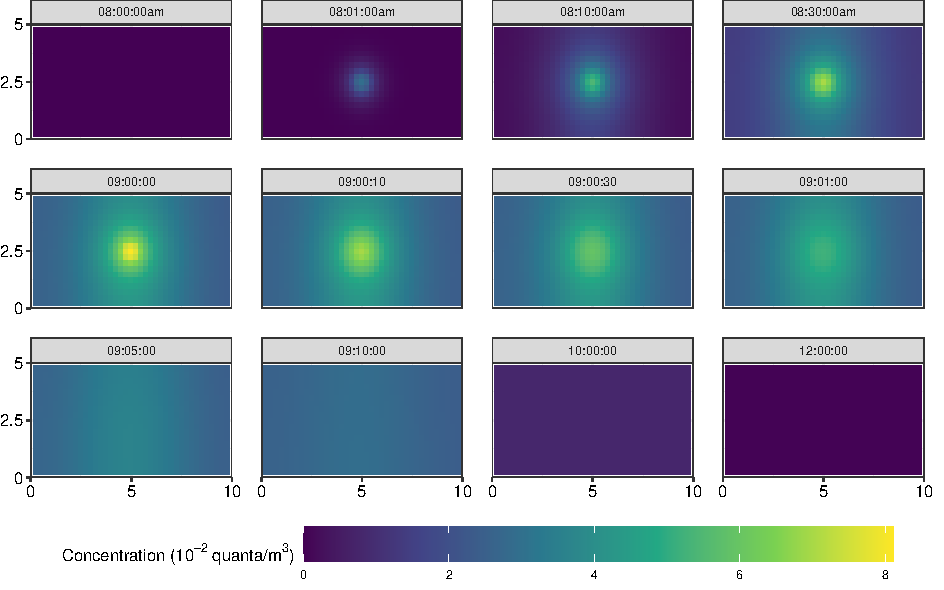
\includegraphics{../../tests/stm_v2-toy_example.pdf}
    \caption{Quanta concentration at different time points following the generation of the first quanta (8:00:00am) and last quanta (9:00:00am) from an infectious individual that is placed in a fixed location in the middle of the room with dimensions L=10m $\times$ B=5m $\times$ H=3m.}
    \label{fig:toy-example}
\end{figure}

\clearpage


\section{Estimation of infection risk in the primary care clinic}\label{sec:estimation}

\subsection{Building and setup}\label{prep:building}

A schematic view of the clinic is shown in \Cref{fig:clinic}. Clinical attendees were tracked when entering the clinic, in the waiting room, the corridor, and the TB room. If they moved into one of the care rooms along the corridor or into other parts of the clinic they were only tracked once they came back. We divide the clinic into three spaces: the waiting room (L=10.55m $\times$ B=5.50m $\times$ H=3.00m), the corridor (L=12.45m $\times$ B=2.20m $\times$ H=2.50m), and the TB room (L=4.75m $\times$ B=3.50m $\times$ H=3.00m). We separated the waiting room and the corridor because we observed small differences in the time-varying CO$_2$ levels, but we acknowledge that the two areas could also be evaluated jointly since the doors to the corridor were often most of the time. Moreover, the corridor and waiting room are not completely enclosed, but connected to the entrance, exit, and other parts of the clinic. Thus, we simplify our modeling analysis when we limit quanta diffusion within these rooms and also note that the calculated air change rate is affected by the separation of the waiting room and corridor (\ie the volume and room occupancy would otherwise be different). 

\begin{figure}[!htpb]
    \centering
    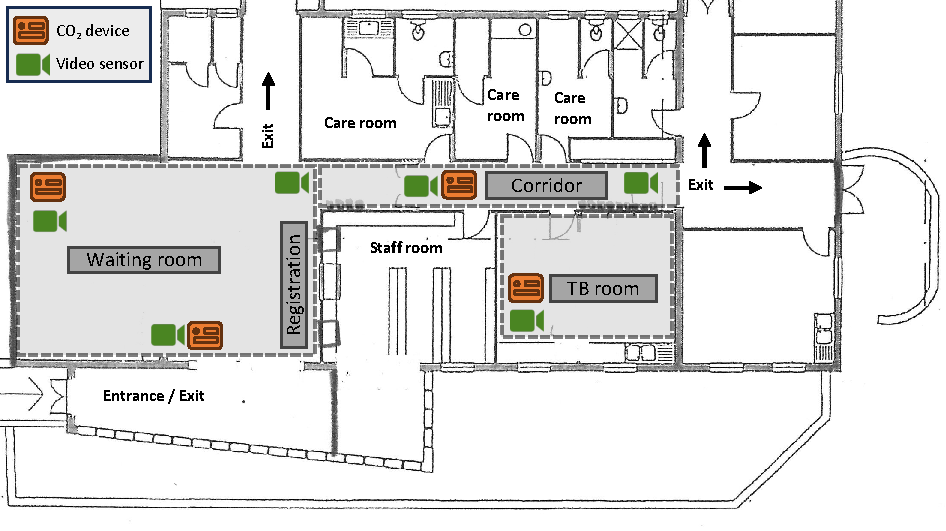
\includegraphics{doc/clinic-schematic-annotated-view.pdf}
    \caption{Schematic view of the part of the clinic where clinical attendees were tracked.}
    \label{fig:clinic}
\end{figure}

As in our illustrative example (\Cref{sec:example}), we divide each room into a grid of cubic cells with dimensions 0.25m$^2 \cdot 3$m, \ie a diagonal length of $\sqrt{0.25^2 + 0.25^2} = 0.35$\,m. Since the rooms have different height, the quanta concentration (quanta/m$^3$) in the corridors' cells will (all else equal) be higher than in the waiting and TB room by a factor of 3/2.5 = 1.2. 

We divide the clinical day into a morning (7am to 12am) and afternoon period (12am to 5pm) and estimate the outdoor air exchange rate separately for each period. Thereby, we allow the $AER$ to vary by daytime, considering potential differences in natural ventilation habits in the morning and afternoon. 

We update the quanta concentration every second at $t = 1, \dots, T$ (aligned with the frequency of the tracking data). We assume that the quanta concentration at $t=0$ is zero anywhere in the airspace, \ie $N_{s,0} = 0 ~~ \forall s$. In other words, we assume that all quanta from the previous day has been removed from the air before the start of the following clinical day. 


\subsection{Monte-Carlo simulation}

We have uncertainty in the data (clinical attendees that are infectious but undiagnosed) and modeling parameters (quanta generation and viral inactivation rate). We consider this uncertainty using Monte-Carlo simulation where uncertain parameters are modeled with prior distributions (see \Cref{sec:priors} below). In each run of the simulation, we perform the following steps:
\begin{itemize}
    \item[\textbf{1.}] Sample uncertain modeling parameters such as the quanta generation rate and the proportion of undiagnosed TB patients among clinical attendees.
    \item[\textbf{2.}] Sample undiagnosed TB patients and combine with diagnosed TB patients, and then use the tracking data to determine the location and time of where and when quanta was generated by these infectious individuals.
    \item[\textbf{3.}] For each room (waiting room, corridor, and passage), compute the quanta concentration in each cell $s$ and at time $t$ using \Cref{eq:spattemp-N} from the spatiotemporal model.
    \item[\textbf{4.}] For each susceptible clinical attendee, compute the risk of infection from the cumulative exposure to quanta over airspace and time using \Cref{eq:spattemp-P}.
\end{itemize}

Most clinical attendees could be undiagnosed TB Patients and there is considerable uncertainty in some modeling parameters. As a consequence, we need a high number of Monte Carlo runs to reasonably estimate the risk of infection for each individual. Therefore, for each study day, we perform 10,000 Monte-Carlo simulations. If not stated otherwise, we summarize the results with the mean and 95\% credible interval. 

\subsection{Prior choices for modeling parameters}\label{sec:priors}

\subsubsection{Initial spread}

% spatial spread of quanta generation

An analysis of exhalation activities suggest a propagation distance (\ie the maximum distance from the source to the end of the exhaled air before dispersion) of 0.7m\cite{Tang2013PLoSOne}, but larger distances may be reached depending on the activity. Face masks reduce the propagation distance both by blocking (the mask capturing particles) and deflecting particles (leakage of particles on the sides of the mask)\cite{Tang2009RoyalInt,Hui2012PLoSOne,Mansour2013AerosolMed}. Therefore, we assume that mask wearing confined the quanta generation only to the cell where the infectious individual is located. This corresponds to a propagation distance of 0.35m (the diagonal cell length) and an area of 0.25$^2$m$^2$. 

To assess the impact of mask wearing, we also model the scenario without mask wearing. In this scenario, we assume a propagation distance of 0.7m (the diagonal lengths of two cells), in line with the aforementioned prior findings. Since we cannot observe the direction of jet, we assume that all neighbouring cells are affected equally. That is, we divide the generated quanta by 9 (the cell where the individual is located and all first-neighbouring cells) and distribute it equally across the cells. 


\subsubsection{Quanta generation rate}

% quanta generation

Previous studies estimated $q$ for \emph{Mtb} or SARS-CoV-2 using the Wells-Riley model\cite{Andrews2014JID,Riley1962ARRD,Escombe2008PLoSMed,Nardell1991ARRD}. Andrews (2014)\cite{Andrews2014JID} reported an estimate of 0.89 quanta/h (range from 0.44 to 5.69), close to the early estimate provided by Riley (1962)\cite{Riley1962ARRD} with 1.25 quanta/h. On the other end, Escombe (2008)\cite{Escombe2008PLoSMed} arrived at an estimate of 8.2 quanta/h, which was lower for non-multidrug-resistant (MDR), smear-negative patients and considerably higher for MDR, smear-positive TB patients. Nardell (1991)\cite{Nardell1991ARRD} also reported a higher estiamte of 13 quanta/h, but only for one index case. The wide range of estimates suggest that the emitted quanta varies considerably with the infectiousness of \emph{Mtb} patients\cite{Wurie2016BMJ}. Therefore, we model $q$ with a Student-t distribution with 1 degree of freedom $t_1(\mu = 2, \sigma = 2.5)$ that is truncated at 0 (lower) and 200 (upper), as in Banholzer (X) [OUR PLOS GLOBAL]. The Student-t distribution with only 1 degree of freedom considers the possibility of superspreaders that generate large amounts of quanta. The distribution function is shown in \Cref{fig:quanta-distribution} along with the estimates from the literature.

\begin{figure}[!htpb]
    \centering
    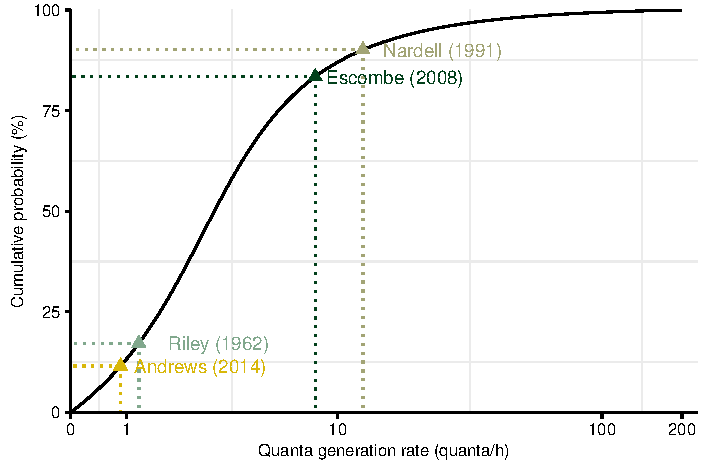
\includegraphics{illustrations/prior-q.pdf}
    \caption{Prior distribution function for the quanta generation rate (quanta/h) along with reported estimates in the literature: 0.89 by Andrews (2014)\cite{Andrews2014JID}, 1.25 by Riley (1962)\cite{Riley1962ARRD}, 8.2 by Escombe (2008)\cite{Escombe2008PLoSMed}, and 13 by Nardell (1991)\cite{Nardell1991ARRD}.}
    \label{fig:quanta-distribution}
\end{figure}

% face mask reduction

Face masks reduce the number of viral-laden aerosols that are exhaled into the air\cite{Milton2013PLoSPathogens,Leung2020NatMed} and should thus lower the generation of infectious quanta. The extent of the reduction is subject to uncertainty. A study with multidrug-resistant TB cases estimated a decrease of 56\% (95\%-CrI, 33\% to 70.5\%) when patients used surgical face masks\cite{Dharmadhikari2012AJRCCM}. This estimate was used by a modelling study to estimate the impact of mask wearing on \emph{Mtb} transmission in a primary care clinic. Therefore, we model the reduction in infectious quanta through mask wearing with a Normal($\mu$ = 0.56, $\sigma$ = 0.11) truncated at 0 and 1. The effective quanta generation rate is thus $q$ times the reduction due to mask wearing. Again, we model what the risk of infection would have been without mask wearing by removing the reduction term from the model. 

\subsubsection{Viral inactivation rate}

% viral inactivation rate

The viral inactivation rate for \emph{Mtb} has not been precisely estimated. Loudon (1969)\cite{Loudon1969AMRRD} report a half-life for aerosolized TB bacilli of 6h ($\lambda$ = 0.12). By contrast, Lever (2000)\cite{Lever2000LettersAppliedMicrobio} reported a half-life of just 5min ($\lambda$ = 8.3). The difference may largely be explained by variation in relative humidity, \ie Loudon (1969) studied survival during a relative humidity of about 50\% whereas Lever (2000) studied survival during a relative humidity of about 70\%. Relative humidity in our study is closer to 50\%, thus the estimate by Loudon (1969) seems more representative of the environmental conditions in our study.  Moreover, Gannon (2007)\cite{Gannon2007ResVetSci} report a half-life of 1.5 hours ($\lambda$ = 0.46) at relative humidity of over 75\%, yet the estimate is for \emph{Mtb bovis}. In contrast to that, Klein (2014)\cite{Klein2014IJMyco} observe a 80\% reduction within 30min ($\lambda$ = 3.2), which would be closer to Lever (2000). We choose a middle ground and, therefore, use a Lognormal($\mu$ = $\log$ 1, $\sigma$ = 1) with a median viral inactivation rate of 1. The distribution function is shown in \Cref{fig:lambda-distribution} along with the estimates from the literature.

\begin{figure}[!htpb]
    \centering
    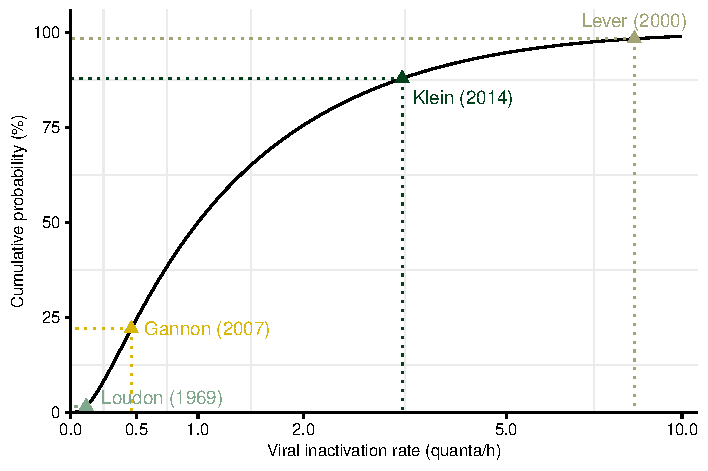
\includegraphics{illustrations/prior-lambda.pdf}
    \caption{Prior distribution function for the viral inactivation rate for \emph{Mtb tuberculosis} along with reported estimates in the literature: 0.12 by Loudon (1969)\cite{Loudon1969AMRRD}, 0.46 by Gannon (2007) for \emph{Mtb bovis}\cite{Gannon2007ResVetSci}, 3.2 by Klein (2014)\cite{Klein2014IJMyco}, and 8.3 by Lever (2000)\cite{Lever2000LettersAppliedMicrobio}.}
    \label{fig:lambda-distribution}
\end{figure}

\subsubsection{Number of undiagnosed TB patients}

% proportion of undiagnosed TB patients

In addition to the diagnosed, known TB patients, there may also be some undiagnosed, unknown TB patients among the clinical attendees. These unmasked TB patients may go undetected because they do not show symptoms according to the WHO 4-question symptom screen (cough, fever, weight loss, and night sweats). A systematic review concluded that half of TB cases among people living with HIV that are on ART may be missed by the symptom screen\cite{Hamada2018LancetHIV}. Similarly, a study universally testing clinical attendees for TB that belong to a risk group (living with HIV, self-reported close contact with TB patients, prior history of TB) finds that 55\% of the attendees without a positive symptom screen were tested positive for TB\cite{Berhanu2023CID}. We interpret these findings such that the number of masked TB patients is roughly equal to the number of unmasked TB patients. On average, there were X masked TB patients per day attending the clinic. Therefore, we model the daily number of unmasked TB patients with a Poisson($\mu$ = X) distribution. 

% based on incidence




\clearpage

\bibliography{references.bib}

\end{document}